% (5-20)

\chapter{Estudo sobre Algoritmos de Agrupamento} \label{cap:estudo}

\begin{section}{Introdução}

No capítulo anterior foi mostrado que pelo menos três modelos geram redes organizadas em módulos que se assemelham a redes de software. Tal resultado favorece o uso dos modelos para avaliar algoritmos de agrupamento de software. Neste capítulo, um dos modelos é usado em um estudo experimental realizado com o propósito de entender melhor os algoritmos de agrupamento apresentados na Seção \ref{sec:algoritmos}.

O estudo experimental foi dividido em duas partes, com dois objetivos distintos:
\begin{enumerate}
	\item comparar o desempenho dos algoritmos de agrupamento sob o critério da semelhança dos agrupamentos encontrados pelos algoritmos com agrupamentos de referência;
	\item entender como o desempenho dos algoritmos é afetado por parâmetros que descrevem cada rede.
\end{enumerate}

Para este estudo foram escolhidos os algoritmos apresentados no Capítulo \ref{cap:agrupamento}: ACDC, Bunch e algoritmos hierárquicos aglomerativos (ligação simples, SL, e ligação completa, CL). Para cada um dos algoritmos aglomerativos, foram estudadas duas alturas de corte, $0,75$ e $0,90$. No total são 4 configurações de algoritmos aglomerativos, que serão referenciadas como SL75, SL90, CL75 e CL90. Para os algoritmos Bunch e ACDC foram escolhidas as configurações padrão das implementações dos autores dos algoritmos. As 6 configurações escolhidas para este estudo são idênticas àquelas estudadas por Wu, Hassan e Holt \cite{Wu2005}.

A fim de simplificar as análises, o estudo experimental foi realizado com redes geradas por apenas um dos modelos apresentados anteriormente, o BCR+. A escolha se deve à familiaridade do autor com as propriedades do modelo. Foram usadas as 9500 configurações de parâmetros descritas no experimento de avaliação de software-realismo, na Seção \ref{sec:parametros}. Para cada configuração foram geradas duas redes a fim de considerar efeitos aleatórios na avaliação dos algoritmos.

% A base dos experimentos são testes de hipótese, nos quais se verificam hipóteses do tipo ``o algoritmo ACDC possui maior desempenho do que o algoritmo CL90''. Verificou-se, no entanto, que a distribuição dos valores de MoJoSim não é normal, o que descarta o teste de t-Student para a comparação de duas amostras. Por essa razão foram utilizados testes não-paramétricos, como o teste de Mann-Whitney, cuja validade não depende da suposição de que a distribuição é normal.

\end{section}

\begin{section}{Comparação entre Algoritmos}

O primeiro experimento teve como objetivo comparar o desempenho dos algoritmos de agrupamento com relação à similaridade entre agrupamentos encontrados pelos algoritmos e os agrupamentos de referência correspondentes.

Cada algoritmo foi aplicado a cada uma das redes sintéticas, resultando em um agrupamento cujo desempenho foi medido pela métrica MoJoSim (ver Seção \ref{sec:fundamentos-avaliacao}). Apenas redes software-realistas (valor $S \ge 0,88$), totalizando XXX redes, foram usadas neste estudo, uma vez que o objetivo é comparar o desempenho de algoritmos quando aplicadas a redes de software.

% XXX falar que quartis são métricas robustas...
A Figura \ref{fig:box-mojo-por-alg} mostra um \emph{boxplot} dos valores de MoJoSim de cada algoritmo. No \emph{boxplot}, o retângulo vai do quartil inferior (Q1) até o quartil superior (Q3), com a mediana desenhada como uma linha horizontal dentro do retângulo. Q1 representa o valor que é maior do que 25\% dos valores, Q3 representa o valor que é maior do que 75\% dos valores. Acima e abaixo do retângulo estão linhas horizontais que indicam o valor mínimo e o valor máximo do conjunto de dados. % As linhas são limitadas por Q1 - (1.5 * IQR) e Q3 + (1.5 * IQR)...

\begin{figure}[htbp]
	\centering
		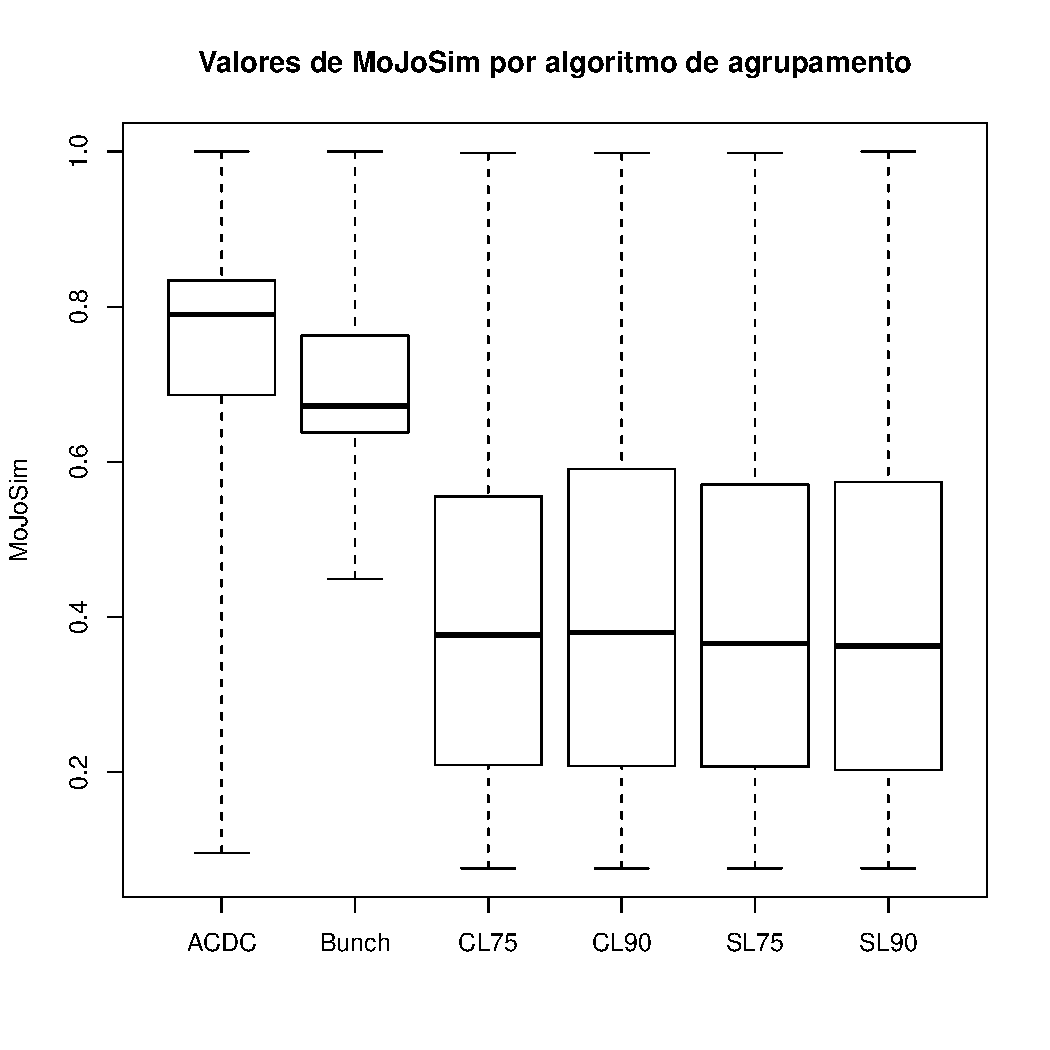
\includegraphics[scale=0.5]{figuras/box-mojo-por-alg}
	\caption{Resumo estatístico dos valores de MoJoSim de cada algoritmo de agrupamento.}
	\label{fig:box-mojo-por-alg}
\end{figure}


Comparando os MoJoSims medianos de cada algoritmo, nota-se que o algoritmo ACDC apresenta o melhor desempenho, seguido do Bunch. A seguir vêm os algoritmos aglomerativos, com pequenas diferenças entre si. A fim de verificar se as diferenças observadas são estatisticamente significativas, foi aplicado o teste de Wilcoxon pareado para cada par de algoritmos, com nível de significância igual a 5\%. O teste confirmou as conclusões feitas a partir do gráfico, mas não encontrou evidências de que algum algoritmo aglomerativo se destaque sobre os demais.

% O teste de Wilcoxon é um teste não paramétrico cuja hipótese nula é a de que, escolhidos dois elementos, um de cada amostra, a probabilidade de que o primeiro seja maior do que o segundo é aproximadamente igual a 50\%. A hipótese alternativa é que os valores de uma amostra tendem a ser maiores do que os valores da outra. Ao contrário do teste de t-Student para comparação de médias de populações, o teste de Wilcoxon não assume que os dados seguem uma distribuição normal.

% Em uma análise complementar, foi selecionado de cada rede o algoritmo de maior desempenho e então contou-se a proporção de redes em que cada algoritmo foi o melhor, como mostra a Figura XXX. Essa análise confirma a superioridade dos algoritmos ACDC e Bunch no conjunto das redes estudadas. Mais do que isso, observa-se que os algoritmos aglomerativos dividem de forma quase igualitária o posto de melhor algoritmo nos casos que não são dominadas pelo ACDC ou pelo Bunch.

Outro aspecto a se observar é a dispersão dos valores. O algoritmo Bunch é o que apresenta a menor dispersão dentre os algoritmos analisados, com mais de 50\% dos valores de MoJoSim na faixa de $0,60$ a $0,80$, e menor MoJoSim igual a $0,45$. No caso do ACDC, 50\% dos valores de MoJoSim estão entre $0,65$ e $0,85$, porém o valor mínimo é $0,01$. Esta observação sugere que o algoritmo Bunch, embora apresente desempenho inferior ao ACDC na maioria dos casos, pode ser uma escolha interessante pelo fato de ter um desempenho mais previsível.

O resultado encontrado diverge das conclusões de Wu, Hassan e Holt \cite{Wu2005}. Eles concluíram que os algoritmos, ordenados do melhor para o pior, são CL90, CL75, Bunch, ACDC, SL75, SL90. As divergências provavelmente se explicam pelos critérios empregados para definir o agrupamento de referência. No estudo deles, o agrupamento de referência foi extraído da estrutura de diretórios do código-fonte dos sistemas estudados; neste estudo, o agrupamento de referência é definido \emph{a priori}, e as redes são geradas de forma a reduzir as dependências entre módulos.

% XXX nível de significância? É assim que se fala?

Vale ressaltar que, apesar de uma amostra grande ter sido usada no estudo, as conclusões não são definitivas. O teste do valor S garante que todas as redes da amostra são software-realistas, mas não é possível afirmar que as redes software realistas estejam bem representadas na amostra. Possivelmente o modelo BCR+ não é capaz de gerar certos tipos de redes software-realistas, o que potencialmente introduz um viés no experimento que pode beneficiar um algoritmo ou outro.

% XXX Defender: ainda assim, esse estudo é ao menos comparável aos estudos de caso que se vê por aí...

\end{section}

\begin{section}{Estudo de Parâmetros}

O segundo experimento teve como objetivo estudar como o desempenho dos algoritmos é afetado pela variação de parâmetros do modelo. Nesse experimento foram usadas todas as redes geradas pelo modelo BCR+, software-realistas ou não.

Este experimento segue um configuração fatorial: são considerados diversos parâmetros, cada um assumindo valores discretos, e as redes assumem todas as combinações possíveis de valores discretos em todos os parâmetros. Tal configuração permite estudar isoladamente o efeito de cada parâmetro sobre o desempenho de um algoritmo.

% A primeira questão estudada foi a seguinte: os algoritmos apresentam melhor desempenho com redes software-realistas? Para responder a essa pergunta, as redes foram divididas em dois grupos (software-realistas e não software-realistas) e os valores de MoJoSim dos grupos foram comparados através do teste de Mann-Whitney (Wilcoxon não-pareado), com 5\% de significância. O teste forneceu evidências de que os algoritmos CL75, CL90, ACDC e Bunch apresentam melhor desempenho quando aplicados a redes software-realistas. O teste foi inconclusivo com relação aos algoritmos SL75 e SL90. As diferenças entre os dois grupos de redes são ilustradas no histograma da Figura XXX.

Um ponto que chamou a atenção foi a relação entre o desempenho dos algoritmos e o número de módulos das redes. Nos algoritmos aglomerativos, um aumento no número de módulos provoca uma piora do desempenho; nos demais algoritmos, não há uma variação significativa. Este fenômeno pode ser observado no gráfico da Figura \ref{fig:mojosim-vs-modules} e foi confirmado através do teste de Wilcoxon pareado com 5\% de significância. Esse é um comportamento, portanto, que diferencia os algoritmos aglomerativos dos demais. 

\begin{figure}[htbp]
	\centering
		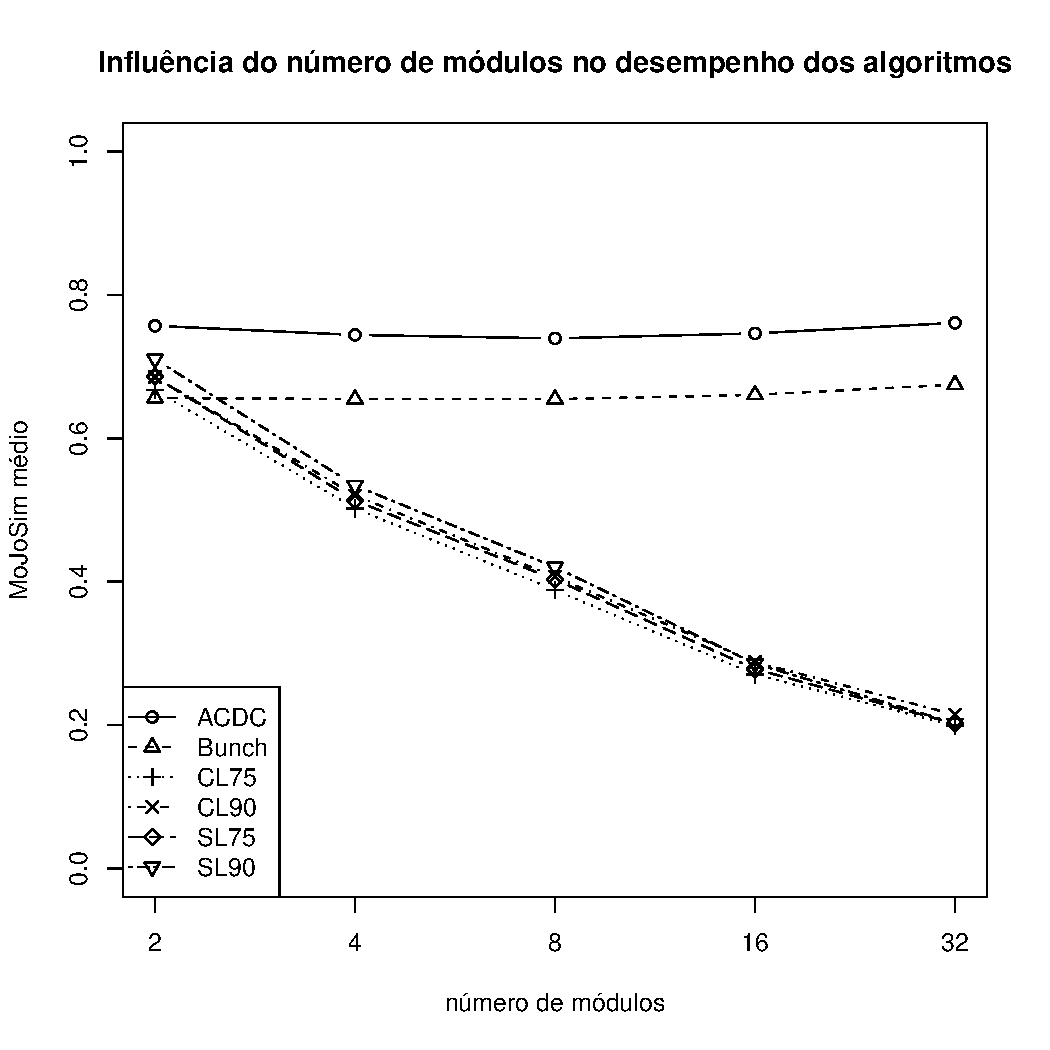
\includegraphics[scale=0.5]{figuras/mojosim-vs-modules}
	\caption{Influência do número de módulos do agrupamento de referência no desempenho de cada algoritmo de agrupamento.}
	\label{fig:mojosim-vs-modules}
\end{figure}

Uma possível explicação está na distribuição dos tamanhos dos módulos encontrados pelos algoritmos aglomerativos. Nestes, é comum serem encontrados módulos muito grandes, às vezes contendo mais da metade da rede. Quando o agrupamento de referência possui muitos módulos, o módulo grande encontrado pelo algoritmo precisa ser dividido em diversos módulos menores, o que a métrica MoJoSim computa como um grande número de operações de mover entidade, penalizando o algoritmo.

% A Tabela XXX mostra o comportamento do desempenho dos algoritmos com o aumento dos valores de cada parâmetro. Em geral, observa-se que o desempenho piora quando os valores dos parâmetros aumentam.

\end{section}

\begin{section}{Conclusão}

Os estudos experimentais descritos neste capítulo mostraram que o algoritmo ACDC apresenta melhor desempenho quando aplicado a redes software-realistas, seguido do algoritmo Bunch, enquanto os algoritmos aglomerativos possuem desempenho inferior. O desempenho dos algoritmos aglomerativos pode, em parte, ser explicado pela sua dificuldade de lidar com redes que possuem muitos módulos. Mostrou-se ainda que os algoritmos CL75, CL90, ACDC e Bunch apresentam desempenho melhor quando aplicados a redes software-realistas.

\end{section}
